\subsection{Skolem functions and regions of validity}
\label{sec:aeval}


%\andreas{I believe the section can be a bit longer. I also think that the keyphrase ``region of validity'' needs to stand out more. Finally, a proof for Lemma 1, or at least an outline of it would be greatly appreciated.}

We rely on the already established algorithm to decide the validity of $\forall\exists$-formulas and extract Skolem functions, called \aeval~\cite{fedyukovich2015automated}.
It takes as input a formula $\forall x \,.\, \exists y  \,.\, \Phi (x, y)$ where $\Phi (x, y)$ is quantifier-free.
To decide its validity, \aeval first normalizes $\Phi (x, y)$ to the form $S(x) \Rightarrow T(x, y)$ and then attempts to extend all models of $S(x)$ to models of $T(x,y)$.
If such an extension is possible, then the input formula is valid, and a relationship between $x$ and $y$ are gathered in a Skolem function.
Otherwise the formula is invalid, and no Skolem function exists.
We refer the reader to~\cite{KatisFGBGW16} for more details on the Skolem-function generation.

Our approach presented in this paper relies on the fact that during each run, \aeval iteratively creates a set of formulas $\{P_i(x)\}$, such that each $P_i(x)$ has a common model with $S(x)$ and $P_i(x) \Rightarrow \exists y \,.\,T (x,y)$.
After $n$ iterations, \aeval establishes a formula $R_n(x) \eqdef \bigvee_{i=1}^n P_i(x)$ which by construction implies $\exists y\,.\,T(x,y)$.
If additionally $S(x)\Rightarrow R_n(x)$, the input formula is valid, and the algorithm terminates.
%
Fig.~\ref{fg:aeval} shows a Venn diagram for an example of the opposite scenario: $R_2(x) = T_1(x) \lor T_2(x)$, but the input formula is invalid.
However, models of each $S(x) \land P_i(x)$ can still be extended to a model of $T(x, y)$.
%Models of $S(x) \land \neg{R_2(x)}$ cannot be extended to models of $T(x,y)$, thus no formula $T_3(x)$ exists, and \aeval terminates.
% \john {Because we are are already using $A$ and $G$ to represent meaningful formulas I suggest that we use different symbols here so it is not confusing. Especially because the symbols have different signatures in these locations.}

In general, if after $n$ iterations $S(x) \land T(x,y) \land \neg R_n(x)$ is unsatisfiable,
then \aeval terminates.
Note that the formula $\forall x.~ S(x) \land R_n(x) \Rightarrow \exists y .~T(x,y)$ is valid by construction at any iteration of the algorithm.
%Thus, a Skolem function can be generated for it.
%Intuitively, a Skolem function
%describes how $y$ is computed from $s$ in order to satisfy the
%previous formula.
%
We say that $R_n(x)$ is a \emph{region of validity}, and in this work, we are interested in the \emph{maximal} regions of validity, i.e., the ones produced by disjoining all $\{P_i(x)\}$ produced by \aeval before termination and by conjoining it with $S(x)$.
Throughout the paper, we assume that all regions of validity are maximal.
% \john{It is a bit strange how we alternate using formulas that have no free variables along with formulas whose free variables are meant to be implicitly existentially quantified. I think we should either stick with a notation or explicitly say that free variables are interpreted to be existentially quantified.}

% \begin{lemma}
% If formula $\forall x \,.\,  S(x) \Rightarrow \exists y . T(x,y)$ is invalid, and $R_n(x)$ is the region of validity, then there is no other formula $S(x)$ such that $S(x) \land R_n(x) \Rightarrow S(x)$ and $\forall x \,.\,  S(x) \Rightarrow \exists y . T(x,y)$.
% \label{lem:subset}
% \end{lemma}

% \begin{proof}
% Suppose that $S(x)$ exists.
% Then $S(x) \land \neg{R_n(x)} \land S(x)$ is satisfiable, and its models are not contained in $R_n(x)$.
% It contradicts our assumption that \aeval has terminated since otherwise it would proceed for generating $T_{n+1}(x)$ which in turn would enlarge the region of validity.
% \end{proof}

\begin{figure}[!t]
\centering
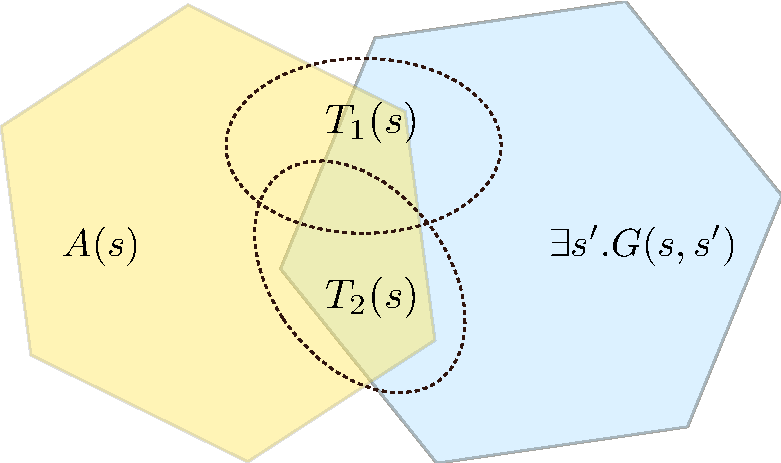
\includegraphics[scale=0.35]{aeval_invalid}
\caption{Region of validity computed for an example requiring \aeval to iterate two times.}
\label{fg:aeval}
\end{figure}

\begin{lemma}\label{lem:aeval}
  Let $R_n(x)$ be the region of validity returned by \aeval for  formula $\forall
  s.~ S(x) \Rightarrow \exists y\,.\,T(x,y)$. Then
%  \begin{equation*}
$  \forall x.~ S(x) \Rightarrow (R_n(x) \Leftrightarrow \exists y\,.\,T(x,y))$.
%  \end{equation*}
\end{lemma}
\begin{proof}
  ($\Rightarrow$) By construction of $R_n(x)$.

  ($\Leftarrow$) Suppose towards contradiction that the formula does
  not hold. Then there exists $x_0$ such that $S(x_0) \land (\exists
  y. T(x_0, y)) \land \neg R_n(x_0)$ holds. But this is a direct
  contradiction for the termination condition for \aeval. Therefore
  the original formula does hold.
\end{proof}

% \begin{corollary}
% If formula $\forall x \,.\,  S(x) \Rightarrow \exists y . T(x,y)$ is invalid, and $R_n(x)$ is the region of validity, then $S(x) \land R_n(x) \Leftrightarrow \exists y . T(x,y)$.
% \label{cor:intermediate}
% \end{corollary}

% \begin{proof}
% ($\Rightarrow$) is immediate from the definition of region of validity.
% ($\Leftarrow$).  Suppose towards contradiction that $s$ satisfies $\exists y . T(x,y)$ but not $S(x) \land R_n(x)$.  If we define $S = s$, we violate Lemma~\ref{lem:subset}.
% \end{proof} 

% \begin{corollary}
% If formula $\forall x \,.\,  S(x) \Rightarrow \exists y . T(x,y)$ is invalid, and $S(x) \land R_n(x)$ is the region of validity, then 
%  $\forall x \,.\, R_n(x) \Leftrightarrow (S(x) \Rightarrow \exists y . T(x,y))$ 
% \label{cor:subset}
% \end{corollary}

% \begin{proof}
% ($\Rightarrow$) Given $s$, suppose $R_n(x)$ is true.  If $S(x)$ is false, then by Corollary~\ref{cor:intermediate},  $\exists y . T(x,y)$ is false, so the implication holds.  Simlarly for $S(x)$ true.
% ($\Leftarrow$) Suppose $S(x) \Rightarrow \exists y . T(x,y)$ is true.  Suppose $S(x)$ is false.  Then $G(s, y)$ might be true and $R_n(x)$ might be false, violating our equivalence.  Boo!
% \end{proof}

